\documentclass[11pt]{article}
\usepackage[letterpaper,margin=0.72in]{geometry}
\usepackage[T1]{fontenc}
\usepackage{lmodern,microtype,graphicx,booktabs,amsmath,array,xcolor,hyperref}
\hypersetup{colorlinks=true,urlcolor=blue,linkcolor=blue,pdfauthor={James N. Jean IV},pdftitle={Freight entry-state substitution under hypothetical constraints}}
\setlength{\parindent}{0pt}
\setlength{\parskip}{6pt}
\renewcommand{\arraystretch}{1.13}
\newcommand{\src}[2]{\href{#1}{#2}}
\begin{document}
{\Large\bfseries Freight entry-state substitution under hypothetical constraints}\par
James N. Jean IV\hfill 29 October 2026\par
\textit{Independent research-program study 08. Not peer reviewed.}

\section*{Decision brief}
Freight continuity plans need to distinguish concentration in estimated flows from evidence that another entry facility and inland route can accept them. We compare a fixed set of state-entry closures in the FAF6.0 2022 water-import-to-truck matrix. Each state denotes its entire entry region, not one port. A closure disables that entry function, not inland deliveries or every road in the state.

\textbf{Conditional finding.} Under 25\% hypothetical additional gateway headroom, strict published origin--entry--destination support and corridor factor 1, recoverable tonnage ranges from 0\% to 100\% across all 16 held commodity/closure cases. This is a finite-model range, not an uncertainty interval, forecast or measured disruption outcome. All 512 declared scenario cases have exact feasible-flow and matching-cut certificates.

\textbf{Practical next step.} Obtain actual facility capacity, physical route feasibility, carrier commitments and disruption timing before making transport commitments. The scenario lattice can structure those questions; it cannot establish available capacity or savings. Each commodity is solved separately and does not establish simultaneous multi-commodity feasibility.

\begin{center}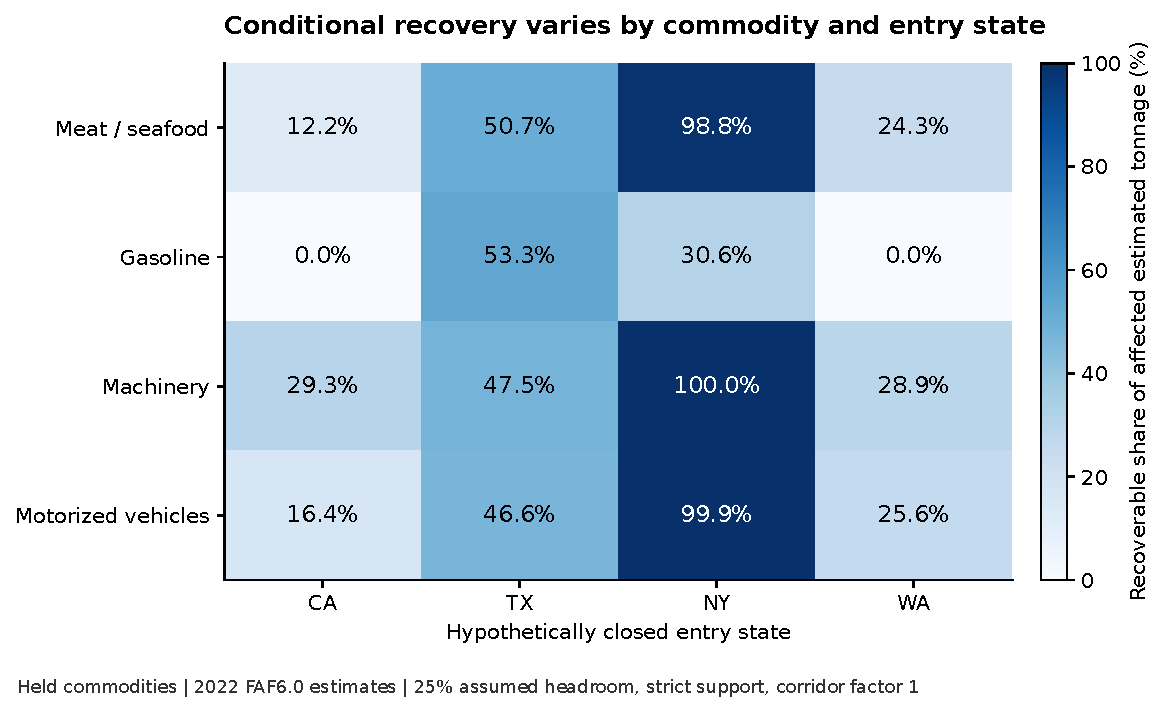
\includegraphics[width=\linewidth]{images/primary_recovery.pdf}\end{center}
\small Figure 1. All held primary cases. Source estimates are in thousand short tons; recovery is a share of affected estimated tonnage. Factors are illustrative and untuned. Exact values and all exclusions are retained.\normalsize

\newpage
\section*{1. Source and prospective design}
The source is the official FAF6.0 state CSV for the 2022 benchmark [1--3]. It contains 599,529 source rows. The fixed filter retains imports (trade type 2), arrival by water (foreign mode 3), domestic truck (mode 1), eight named SCTG commodities, all eight foreign-origin regions and all 51 state/DC destinations. The selected projection contains 8,563 estimated-flow cells, no duplicate source-dimension keys and no selected zero rows. Missing cells mean no published support in this selected matrix; they do not prove physical impossibility.

The initial public protocol commit \texttt{adcdd61} precedes archive retrieval. Header-only inspection found state-field aliases \texttt{dms\_origst}, \texttt{dms\_destst} and \texttt{tons\_2022}; the public schema clarification \texttt{c5ba860} precedes value inspection. The included metadata specifies \textbf{thousand short tons}. The selected source facts preserve every original dimension, original decimal tonnage, CSV row locator and selected-field SHA-256. Monetary values, full archives, source workbooks and unrelated commodities are excluded from public Git. Source citation accompanies the derivative; no agency endorsement is implied.

\begin{center}\small
\begin{tabular}{lll}\toprule
Phase & Fixed SCTG codes & Descriptions\\\midrule
Development & 02, 12, 24, 32 & Cereal grains; gravel; plastics/rubber; base metals\\
Held & 05, 17, 34, 36 & Meat/seafood; gasoline; machinery; motorized vehicles\\\bottomrule
\end{tabular}\end{center}

Close California (06), Texas (48), New York (36) and Washington (53) separately. Additional gateway headroom is 0, 1/4, 1/2 or 1 times estimated baseline flow. Corridor multiplier is 1/4 or 1; support is strict or pooled. This yields 512 cases: 256 development and 256 held. The primary setting is fixed at headroom 1/4, corridor factor 1, strict support. No commodity, state, factor, outcome or baseline was selected from held summaries. These choices define a finite illustrative design rather than a representative sample.

\textbf{Separation.} Twelve fixtures and all development checks passed before the public freeze \texttt{3179c9a}. That freeze records 17 canonical dependencies from analysis/source commit \texttt{bab87e6}. Held analytical summaries were then computed unchanged. All raw source rows and source-quality information were accessible, so this is an execution separation without blinding, fitting or a predictive-generalization claim. There was no parameter search or random computation.

\textbf{Independent source checks.} Positional parsing, exact SQL grouping and a second CSV engine reconcile the projection to the complete official member. The independent engine verifies 102,756 selected fields, row locators and digests; the public projection checker performs 85,632 checks. Archive and member SHA-256 values are retained in the source manifest. Hash identity certifies the inspected bytes, not the truth of estimated freight or current traffic conditions. FAF limitations include local detail and road coverage; operator consultation is necessary [2].

\newpage
\section*{2. Allocation model and finite-model optimality}
For a separately solved commodity, let $F_{ogd}$ be the published estimate from foreign region $o$ through entry state $g$ to domestic destination $d$. Closing $g_0$ defines affected demand $D_{od}=F_{og_0d}$. Alternative entries exclude $g_0$. The objective is maximum recovered affected tonnage, with all original origins and destinations preserved.

\begin{center}\small
\begin{tabular}{p{.31\linewidth}p{.60\linewidth}}\toprule
Directed edge & Hypothetical capacity\\\midrule
Source to entry $g$ & $\delta\sum_{o,d}F_{ogd}$, a shared additional-flow headroom convention\\
Entry $g$ to origin/entry $(o,g)$ & $\sum_d F_{ogd}$, a fixed 100\% additional-flow cap\\
$(o,g)$ to origin/destination $(o,d)$ & Strict: $\beta F_{ogd}$. Pooled: $\beta\sum_{o'}F_{o'gd}$. Require positive origin/entry support and affected demand.\\
$(o,d)$ to sink & $D_{od}$\\\bottomrule
\end{tabular}\end{center}

The shared gateway limit and corridor limits differ; headroom is not automatically a uniform rescaling of every edge. Pooled support permits substitution of a domestic corridor observed for another foreign origin, while still requiring positive origin/entry baseline support and preserving the affected origin. It is a relaxed assumption, not a verified service link. In either support convention, no physical port, ocean schedule or road path is reconstructed. The graph reallocates an aggregate flow estimate.

Published decimal strings and factors are represented as exact fractions and scaled to integer ticks. An original residual level-graph implementation allows prior allocations to be reversed when another path increases feasible recovery. Decimal precision avoids arithmetic ambiguity; it does not establish physical measurement precision. The baseline with no rerouting recovers zero. A second feasible baseline visits foreign origin, destination and alternative gateway in ascending numeric order, consuming remaining shared, origin/gateway, corridor and demand capacities. Its order is fixed and is not claimed to be an optimized operational policy.

An independent checker does not import production graph, solver or greedy helpers. It reconstructs every capacity from the source-derived SQL cells; verifies nonnegative flows, each capacity and internal-node conservation; and requires source/sink flow value to equal the capacity of a separately reconstructed source--sink cut. Feasible flow plus an equal-capacity cut certifies optimality for that graph [4]. Residual reachability is independently checked, and greedy allocations are independently reconstructed. This proves finite-model optimality, not operational feasibility.

Twelve fixtures include exhaustive tiny-cut enumeration, reverse-flow reallocation, disconnected and zero-flow cases, shared capacities, fractional scaling, large integer arithmetic, support expansion, an origin-specific bottleneck and a greedy counterexample. All 512 cases remain available with positive-flow records, cut node sets, integer scale and original per-case computation times. No failed numerical scenario was omitted.

\newpage
\section*{3. Complete held primary comparison}
Table 1 retains every held commodity/closure case at the fixed primary setting: $\delta=1/4$, $\beta=1$, strict support. Each is a separate scenario; their affected quantities must not be interpreted as one simultaneous disruption. Every affected quantity is positive in this source snapshot. The protocol would retain a zero-demand case with an undefined recovery share.

\begin{center}\small
\setlength{\tabcolsep}{3.3pt}
\begin{tabular}{llrrrrr}\toprule
Commodity & Entry & Affected & Recovered & Unmet & Share (\%) & Gain\\\midrule
Meat/seafood & CA & 415.170 & 50.600 & 364.570 & 12.2 & 0.000 \\
Meat/seafood & TX & 55.364 & 28.074 & 27.290 & 50.7 & 0.000 \\
Meat/seafood & NY & 108.466 & 107.140 & 1.326 & 98.8 & 0.000 \\
Meat/seafood & WA & 126.732 & 30.755 & 95.977 & 24.3 & 0.000 \\
Gasoline & CA & 4,271.198 & 0.000 & 4,271.198 & 0.0 & 0.000 \\
Gasoline & TX & 628.892 & 335.501 & 293.391 & 53.3 & 0.000 \\
Gasoline & NY & 450.181 & 137.627 & 312.554 & 30.6 & 0.000 \\
Gasoline & WA & 257.180 & 0.000 & 257.180 & 0.0 & 0.000 \\
Machinery & CA & 4,181.086 & 1,226.016 & 2,955.069 & 29.3 & 14.227 \\
Machinery & TX & 778.736 & 369.655 & 409.081 & 47.5 & 0.000 \\
Machinery & NY & 100.588 & 100.588 & 0.000 & 100.0 & 0.000 \\
Machinery & WA & 861.181 & 248.642 & 612.539 & 28.9 & 0.000 \\
Motorized vehicles & CA & 6,222.386 & 1,020.410 & 5,201.976 & 16.4 & 14.418 \\
Motorized vehicles & TX & 357.348 & 166.521 & 190.827 & 46.6 & 0.000 \\
Motorized vehicles & NY & 16.878 & 16.855 & 0.023 & 99.9 & 0.000 \\
Motorized vehicles & WA & 892.154 & 228.810 & 663.344 & 25.6 & 0.015 \\
\bottomrule\end{tabular}\end{center}
\small Table 1. Affected, recovered, unmet and gain columns are thousand short tons, rounded to three decimals for display. Gain is optimal recovery minus fixed feasible greedy recovery under the same constraints. Shares are rounded to one decimal. Exact rational values are in \texttt{results/held.csv}. Neither rounding nor retained source decimals convey physical precision.\normalsize

The complete range spans zero recovery and complete recovery under the declared model. Zero recovery in California and Washington gasoline cases results from the selected support/capacity conventions; it does not prove that a real route cannot be arranged. New York machinery reaches 100\% in this scenario; it does not prove that real facilities or carriers can accept that volume.

The optimizer improves on the deterministic baseline in 3 of the 16 primary cases and ties in 13. The primary gains are 14.227, 14.418 and 0.015 thousand short tons after display rounding. These are conditional allocation differences. They are not measured shipments, capacity additions or realized savings. The exact solver establishes the best feasible allocation in the specified graph, while the constraints themselves remain hypothetical.

\newpage
\section*{4. Sensitivity across the retained design}
\begin{center}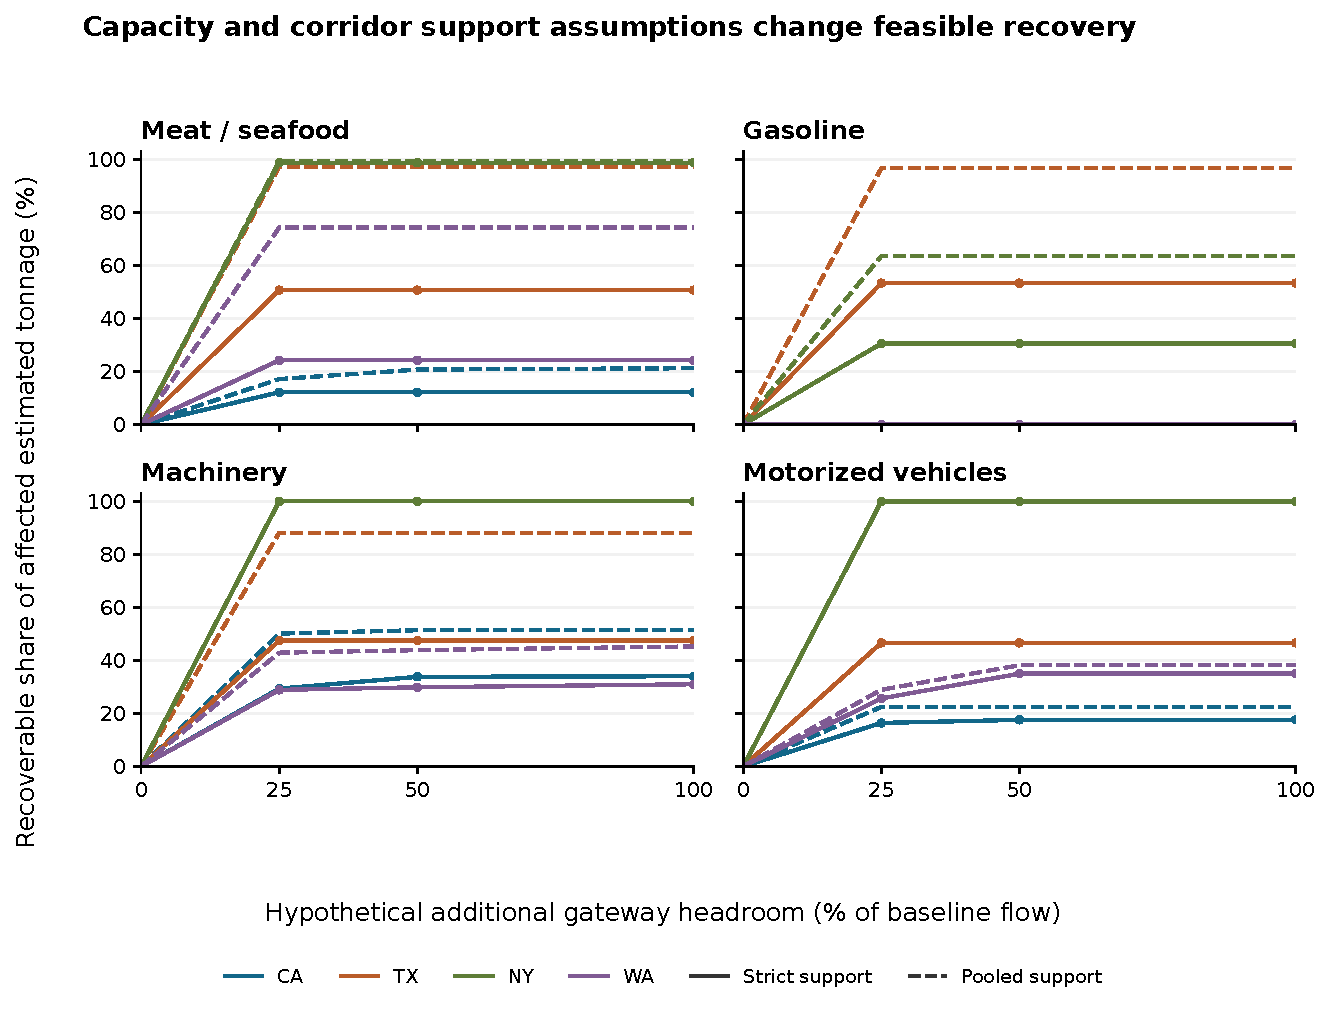
\includegraphics[width=\linewidth]{images/headroom_sensitivity.pdf}\end{center}
\small Figure 2. All four closures and all four headroom factors for each held commodity at corridor factor 1. Solid lines use strict origin-specific support; dashed lines use pooled destination-corridor support. Headroom is hypothetical additional capacity relative to baseline estimated flow. Connecting grid points guides reading; no interpolation was evaluated. The complete exported lattice also retains corridor factor 1/4.\normalsize

Recovery cannot decline when a declared capacity increases or a feasible edge set expands. Independent checks verify 1,152 such comparisons per phase, 2,304 in total. This is a finite-model consistency property, not independent empirical evidence that physical recovery increases by the same amount. Some curves plateau because another declared constraint binds.

Across all 256 held cases, exact optimization improves on the fixed greedy allocation in 27 and ties in 229. The largest declared-lattice gain is 70.630 thousand short tons after rounding. We do not search alternative greedy orders or claim that this baseline exhausts practical policies. There is no predictive score, calibrated probability, confidence interval, p-value or causal comparison. The source does not supply uncertainty intervals for these selected cells, and no sampling mechanism justifies treating this lattice as repeated empirical disruptions.

\newpage
\section*{5. Algorithm comparison and planning limits}
\begin{center}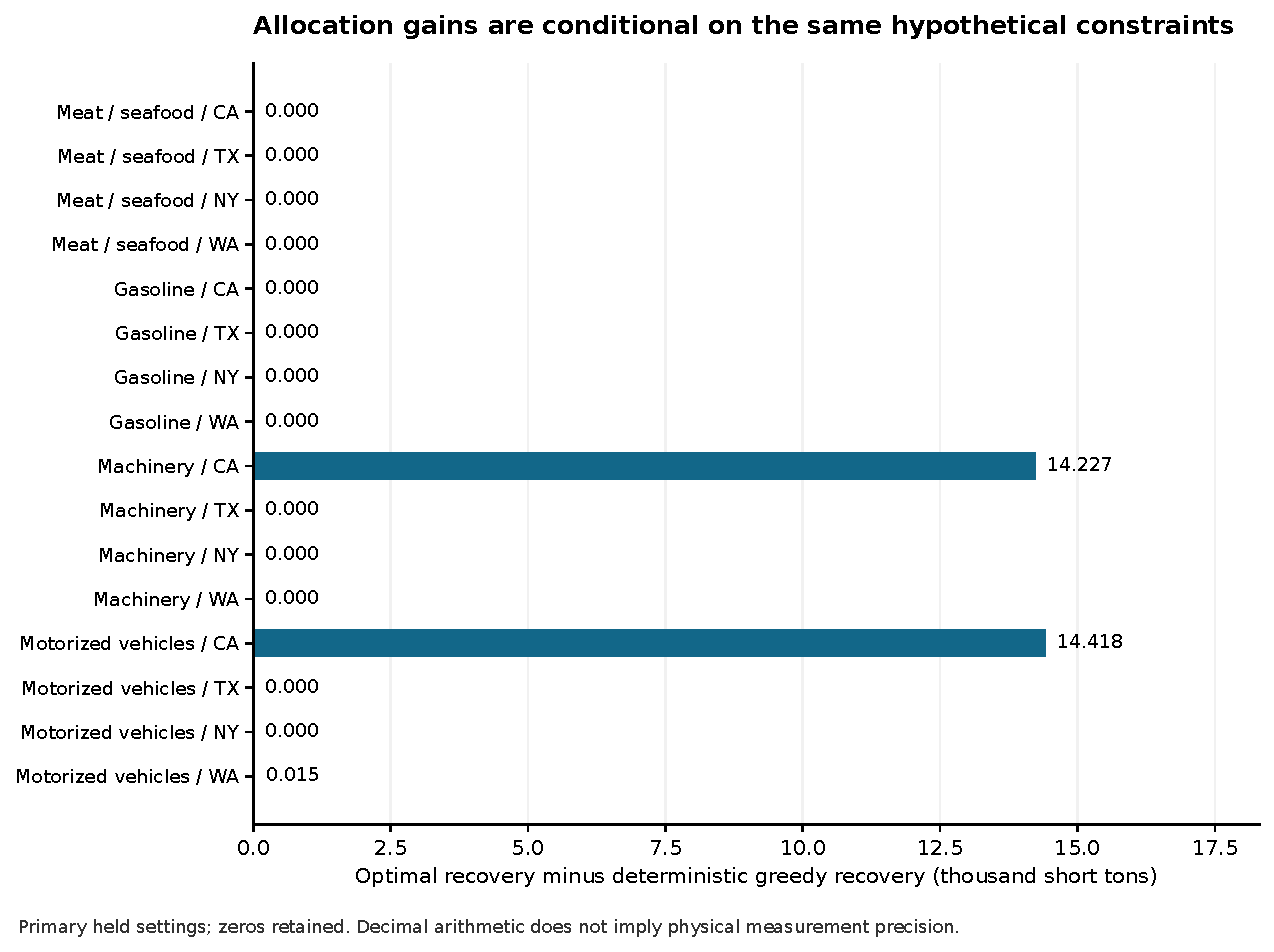
\includegraphics[width=.96\linewidth]{images/greedy_gap.pdf}\end{center}
\small Figure 3. All 16 held primary optimizer--greedy gaps, including zero gains. The units are thousand short tons of conditional allocation under identical constraints. This is not a monetary or realized-benefit chart.\normalsize

The source lacks actual spare capacity, entry-facility and road topology, ocean or inland timetable, contracts, commodity handling compatibility and observed disruption response. Origin/gateway and corridor factors are illustrative conventions without empirical calibration. The selected state/commodity set does not establish broad geographic or product representativeness. Separate commodity solves omit competition for shared physical resources. Exact arithmetic and optimization cannot repair these missing operational inputs.

\newpage
\section*{6. Reproducibility and evidence status}
The isolated replay reproduces 759,047 exact CSV and certificate scalar fields across both phases and rechecks the 17 frozen dependencies. Independent result checks total 813,520 development and 934,029 held exact checks, or 1,747,549 combined, plus 2,304 monotonicity checks. The original execution records retain per-case UTC timestamps and elapsed seconds. Replay timings vary and are excluded from output identity. No random seed is needed because all computations and orders are deterministic.

Three original figures are checked against independent fractions from the exported results: 288 actual artist values, 16 heatmap annotations and 16 foreground-contrast checks with a minimum ratio of 4.5. These checks do not establish accessibility conformance. The manuscript and all pages are rendered and inspected separately. Public-file hashes, source provenance and independent checks support the scoped claim; source accuracy and operational feasibility remain unestablished.

\textbf{Reproduction commands} (from the repository root):
\begin{quote}\small\ttfamily
python -m pip install -r requirements.txt\par
python -m unittest discover -s tests -v\par
python src/check\_reproduction.py\par
python src/verify\_figures.py\par
python src/verify\_paper.py\par
python src/verify\_public\_package.py
\end{quote}
The selected projection is sufficient for public replay. The source manifest and retained raw reconciliation receipt document the completed archive check; CI does not silently substitute a later release. Full source archives, workbooks and third-party documents stay outside public Git. Separate projects intended for formal publication, including Azure optimization, are excluded. This independent program manuscript is not peer reviewed, introduces no new estimator or algorithm, and makes no exhaustive novelty claim.

\textbf{Recommendation.} Use the conditional lattice to prioritize questions for facilities, carriers and infrastructure owners. Replace or justify the capacity/support assumptions with authorized operational evidence before committing to a substitute flow. A new source version or revised operational model requires a separately labeled protocol and validation; the current frozen results should remain inspectable.

\section*{References}
\small
[1] U.S. Department of Transportation, Bureau of Transportation Statistics. \textit{Freight Analysis Framework, FAF6 datasets}, 2022 benchmark, version 6.0. \src{https://doi.org/10.21949/fhgm-g335}{Dataset DOI}; \src{https://www.bts.gov/faf}{official download page}. Accessed 29 October 2026.\par
[2] Bureau of Transportation Statistics. \textit{FAF FAQs and Limitations}. \src{https://www.bts.gov/faf/faqs}{Official limitations and recommended operator consultation}.\par
[3] Bureau of Transportation Statistics. \textit{Freight Analysis Framework Version 6 User's Guide}, July 2026; included FAF6 metadata workbook. \src{https://faf.ornl.gov/faf6/data/FAF6\%20User\%20Guide.pdf}{Guide}; source archive and exact SHA-256 in the repository manifest.\par
[4] MIT 6.854. \textit{Lecture 7: Basic Flow Algorithms and Capacity Scaling}, 2019. \src{https://courses.csail.mit.edu/6.854/19/Notes/n07-flow_computation.html}{Flow/cut optimality conditions}. Established method; original implementation here.
\end{document}
